\documentclass{beamer}

\usepackage[utf8]{inputenc}


\usepackage{tikz,amsmath, amssymb,bm,color}
\usetikzlibrary{overlay-beamer-styles}

\tikzstyle{normal}=[circle,fill=white, draw=black, thick]

\usetheme{Madrid}

\usepackage[en-NZ]{datetime2}
\DTMlangsetup{showdayofmonth=false}

%Information to be included in the title page:
\title[The Colouring Game and the Activ. Strat.]{The Colouring Game and the Activation Strategy}
\author{Matthew Askes}
\institute[Victoria University]{Victoria University of Wellington}
\date{\today}


\begin{document}

\frame{\titlepage}

%-------------------------------frame 0------------------------------------------

\begin{frame}{Outline}
    \tableofcontents
\end{frame}

%###############################Introduction#####################################
\section{Introduction}

%-------------------------------frame 1------------------------------------------

\begin{frame}{\secname}{What is a Graph?}
    %definations 1.
      
    \begin{columns}
        \begin{column}{0.7\textwidth}
             A graph, $G=(V,E)$, is a pair consisting of objects and a relation on these objects. The objects are called vertices and the set of all vertices is denoted $V$. E.g. $a,b,c$ are vertices in the figure.
             
            \bigskip
            
            The relation is represented as pairs of vertices called edges. The set of all edges is denoted $E$. E.g. $(a,b)$ and $(c,a)$ are edges in the figure.
        \end{column}
        \begin{column}{0.3\textwidth}  
            \begin{center}
                \begin{figure}[h]
                    \centering
                    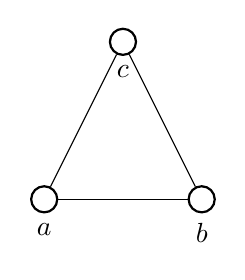
\begin{tikzpicture}[scale=2]
                    \node[normal, label=below:$a$] (v1) at (-1.5,-1) {};
                    \node[normal, label=below:$b$] (v3) at (-0.5,-1) {};
                    \node[normal, label=below:$c$] (v2) at (-1,0) {};  
                    \draw (v1) edge (v2);
                    \draw  (v2) edge (v3);
                    \draw  (v3) edge (v1);
                    \end{tikzpicture}
                    \caption{An graph with three vertices and three edges}
                    \label{fig:k3}
                \end{figure}
            \end{center}
        \end{column}
    \end{columns}
    
\end{frame}

%-------------------------------frame 2------------------------------------------

\begin{frame}{\secname}{What is a Graph Colouring?}
    %definations 2.
    
    Let $C=\{1,\dots,k\}$ be a set of colours, a \textit{$k$--vertex colouring} of a graph $G=(V,E)$ is a mapping $c\colon V \to C$. 
    
    \bigskip
    
    A \textit{proper $k$--vertex colouring} of $G$ is a colouring such that for two vertices $u,v\in V$ if $(u,v)\in E(G)$ then $c(u)\neq c(v)$.
    
    \bigskip
    %chromatic number 3. 
    
    The \textit{chromatic number}, $\chi(G)$, of a graph $G$ is the smallest $k$ such that $G$ has a proper $k$--vertex colouring.
\end{frame}


%###############################The Colouring Game###############################
\section{The Colouring Game}

%-------------------------------frame 3------------------------------------------

\begin{frame}{\secname} 
        
    %introduce col. game 4.
        
    %defination 5.
    
    The game is played between two players, Alice and Bob.
    
    \bigskip
    
    Let $G$ be a graph, and $C$ a set of colours. Beginning with Alice, Alice and Bob take alternating turns. On their turn they choose an uncoloured vertex, $v$, and assign $v$ a colour from $C$ such that no two adjacent vertices in $G$ have the same colour. 
    
    \bigskip
    
    This continues until one of two win conditions are meet. First, Alice wins if all the vertices are coloured. Second, Bob wins if there is a vertex that cannot be coloured with the available colours.
\end{frame}

%-------------------------------frame 4------------------------------------------

\begin{frame}{\secname}{Have a go}
    
    %play with the audiance 6.
    
    Any volunteers to play this game?
    
    \bigskip
    
    You play as Bob. Your goal is to prevent the graph from being coloured.
    
    %todo link to game
\end{frame}

%-------------------------------frame 5------------------------------------------

\begin{frame}{\secname}{An Unwinnable Game}
    
    %why they cannot win? 7.
    
    The volunteers were unable to prevent the graph from being coloured. Why?
    
    \bigskip
    
    In short, there were too few colours.
    
    %colouring number 8.
    
    \bigskip
    \pause
    
    \begin{block}{Defination}
        For a graph $G$ the \textit{game chromatic number}, $\chi_g(G)$, is the smallest number of colours needed to guarantee that Alice has a winning strategy on $G$, when playing the colouring game in $G$.
    \end{block}
   
\end{frame}

\begin{frame}{\secname}{How many colours is enough?}
    Trivial bounds for the colouring number,$\chi_g(G)$, on $G=(V,E)$:
    \[\chi(G) \leq \chi_g(G) \leq |V|\]
    
    \bigskip
    
    For a better bound we need a strategy for Alice.
    
    \bigskip
    \pause
    
    Such a strategy is the \textit{Activation Strategy}.
\end{frame}


%###############################Activation Strategy##############################
\section{Activation Strategy}

%-------------------------------frame 6------------------------------------------

\begin{frame}{\secname}
    %explain stategy 9.
    Fix a graph $G$ and a linear order $L$ on $V$. We keep track of a set of activated vertices $A$. Alice plays activation strategy is played as follows,
    \begin{enumerate}
        \item Alice starts by colouring and activating the least vertex in the ordering $L$.
        \item On her next turn, let $u$ be the last vertex marked by Bob.  Alice starts at $u$ activates it and moves to the least uncoloured out--neighbour of $v$, $w$. \label{enum:actvstrat}
        \item If $w$ is activated then Alice stops and colours $w$. If not, then Alice repeats from step (\ref{enum:actvstrat}) on $w$ instead of $u$. 
        This continues until Alice lands on a vertex $x$ that is activated or has no uncoloured out--neighbours. Alice colours $x$.
        \item If the last vertex marked by Bob has no uncoloured out--neigbbours, then Alice colours and activates the least uncoloured vertex in the ordering $L$.
    \end{enumerate}
\end{frame}

%-------------------------------frame 7------------------------------------------

\begin{frame}{\secname}{Graph Matchings}
    %we bound col. num. using actv. strat. 10.
    
    % graph rank 11.
    
    \begin{definition}[Matching]
        Let $G$ be a graph. A \textit{matching} $M\subset E(G)$ is a set of independent edges, that is a set of edges that share no common vertices.\\
        
         We say $M$ is a matching from $X$ to $Y$ if $X,Y\subseteq V(G)$ and all the edges in $M$ connect a vertex in $X$ to a vertex in $Y$. That is if $(u,v)\in M$ then $u\in X$ and $v\in Y$. 
        
    \end{definition}

\end{frame}

\begin{frame}{\secname}{Graph Rank}
    %we bound col. num. using actv. strat. 10.
    
    % graph rank 11.
    
    \begin{definition}[Graph Rank]   
    Let $G$ be a graph and $L$ a linear order on $V(G)$.
    
    For $u \in V(G)$ the \textit{matching number} $m(u, L, G)$ of $u$ with respect to $L$ in $G$ is defined to be the size of the largest set $Z \subset N^-[u]$ such that there exists a partition $\{X, Y\}$ of $Z$ and there exist matchings $M$ from
    $X\subset N^-[u]$ to $V^+(u)$ and $N$ from $Y\subset N^-(u)$ to $V^+[u]$.
    
    The rank $r(L,G)$ and rank $r(G)$ are defined as:
    \begin{align*}
    r(u,L,G) & = d^+_{G_L}(u) + m(u,L,G) \\
    r(L,G)   & = \max_{u \in V}r(u,L,G)  
    \end{align*}
\end{definition}
\end{frame}

%-------------------------------frame 8------------------------------------------

\begin{frame}{\secname}{Upper Bound Using Activation Strategy}
    %auctal bound (thm) 12.
    
    \begin{block}{Theorem [Kierstead 2000]}
        For any graph $G$ and linear ordering $L$ on $V(G)$, if Alice uses the activation strategy to play the colouring game on $G$, then she will win if there are at least $1+r(L, G)$ colours. In particular, $\chi_g(G) \leq 1+r(L, G)$.
    \end{block}
\end{frame}

%-------------------------------frame 9------------------------------------------

\begin{frame}{\secname}{Treewidth and Pathwidth Definitions}
    %Treewidth and pathwidth and their linear orders 13., 14.
    
    
    A tree decomposition $(X,T)$ of a graph $G$ is a tree, $T$, along a collection of subsets of $V(G)$, $X=\{X_1,\dots,X_n\}$, indexed by vertices in $T$, such that $V(G)=\bigcup X$ and obeys the following properties.
    \begin{enumerate}[(i)]
        \item For all edges $(u,v)$ in $E(G)$ there exists an $i$ such that $u,v\in X_i$
        \item  If there exists an $x,y\in V(T)$ and vertices $u,v$ such that $v\in X_x$ and $v\in X_y$ then for all $l$ on the path from $x$ to $y$ $v\in P_l$.
    \end{enumerate} 
    The width of a tree decomposition is the maximum value of $|X_i| -1$ for all $i\in V(T)$.

    
    \begin{definition}[Treewidth]
        The \textit{treewidth} of a graph $G$ is the minimum width of a tree decomposition of $G$.    
        A graph of bounded treewidth, $k$, is a graph with treewidth less than or equal to $k$. 
    \end{definition}
    
\end{frame}

%-------------------------------frame 10------------------------------------------

\begin{frame}{\secname}{Treewidth and Pathwidth Bounds}
    %bounds for treewidth, pathwidth, trees, ?planar graphs?, 15.
    Some bounds using the activation strategy are as follows,
    \begin{itemize}
        \item For a tree $T$ \begin{flalign*}
            &&\chi_g(T) = 4 && \text{[Kierstead 2000]}
        \end{flalign*}
        \pause
        \item For $G$ a graph of pathwidth $k$\begin{flalign*}
       & &\chi_g(G) \leq 3k + 1\ && \text{[Bodlaender 1998]]}
        \end{flalign*}
        \pause
        \item For $G$ a graph of treewidth $k$\begin{flalign*}
        & &\chi_g(G) \leq 3k + 2\ && \text{[Wu, Zhu 2008]]}
        \end{flalign*}
    \end{itemize}
    
\end{frame}


%##############################Other Graph Games##################################
\section{Other Graph Games}

%-------------------------------frame 11------------------------------------------

\begin{frame}{\secname}
    %Other games 16.
        % marking game 17.
        % other col. strat. and col. extensions 18.
        % dom. game 19.
        % ind. dom. game. 20
    j
\end{frame}
\end{document}











